% SOMA gate architecture (inference).
% Solid path is the deployed system. Dashed = 32B teacher, train-time only.
% No MiniLM, emotion, PPO, or extra modules.
\documentclass[tikz,border=7pt]{standalone}
\usepackage[T1]{fontenc}
\usepackage[scaled=0.92]{helvet}
\renewcommand{\familydefault}{\sfdefault}
\usepackage{tikz}
\usetikzlibrary{arrows.meta,positioning,calc}

\definecolor{ink}{HTML}{1E2933}
\definecolor{steel}{HTML}{2E6FA8}
\definecolor{ochre}{HTML}{C17B24}
\definecolor{pine}{HTML}{1A8F5C}
\definecolor{slate}{HTML}{4F6F8F}

\begin{document}
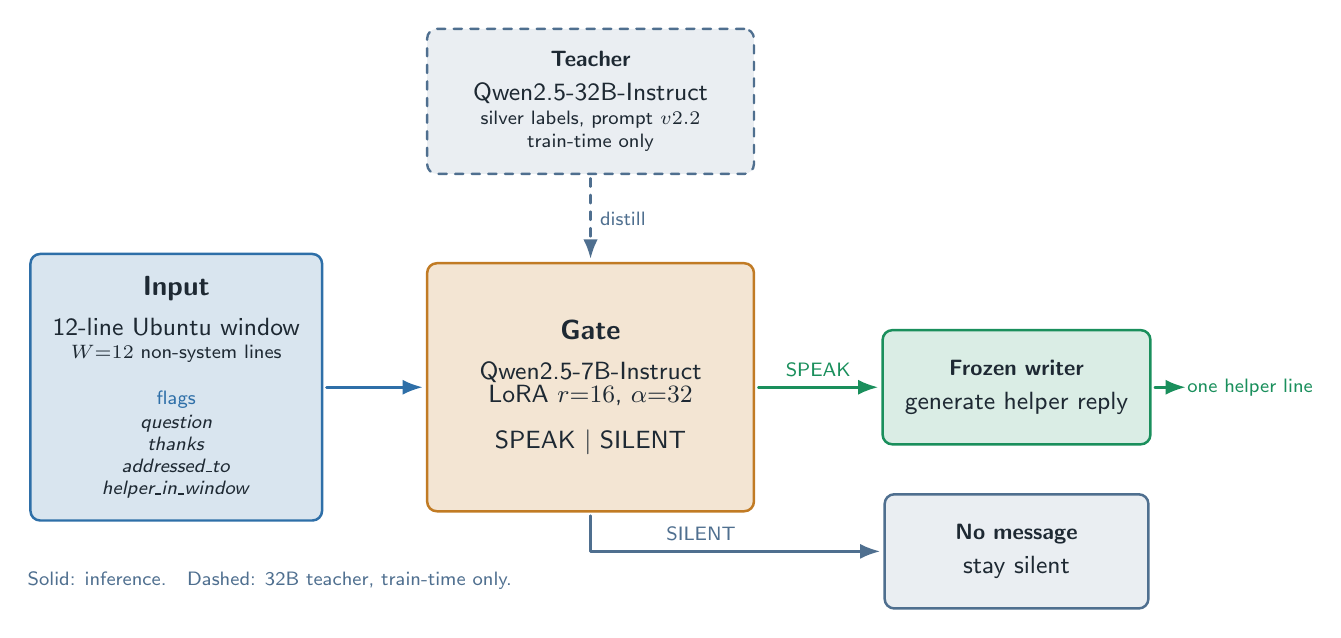
\begin{tikzpicture}[
  font=\sffamily\footnotesize,
  line cap=round,
  line join=round,
  >=Latex,
  every node/.style={
    align=center,
    text=ink,
  },
  box/.style={
    rounded corners=3.5pt,
    line width=0.9pt,
    inner sep=8pt,
    outer sep=1.2pt,
    minimum width=3.55cm,
  },
  inbox/.style={
    box,
    draw=steel,
    fill=steel!18,
    minimum height=3.15cm,
  },
  gatebox/.style={
    box,
    draw=ochre,
    fill=ochre!20,
    minimum width=4.15cm,
    minimum height=3.15cm,
  },
  tchbox/.style={
    box,
    draw=slate,
    fill=slate!12,
    dashed,
    line width=0.85pt,
    minimum width=4.15cm,
  },
  wrbox/.style={
    box,
    draw=pine,
    fill=pine!16,
    minimum width=3.35cm,
    minimum height=1.45cm,
  },
  slbox/.style={
    box,
    draw=slate,
    fill=slate!12,
    minimum width=3.35cm,
    minimum height=1.45cm,
  },
  arr/.style={
    ->,
    steel,
    line width=0.95pt,
    shorten >=0.4pt,
    shorten <=0.4pt,
  },
  dasharr/.style={
    ->,
    slate,
    dashed,
    line width=0.9pt,
    shorten >=0.4pt,
    shorten <=0.4pt,
  },
]

% --- nodes ---
\node[inbox] (in) {
  {\bfseries\normalsize Input}\\[5pt]
  {\small 12-line Ubuntu window}\\[-1pt]
  {\scriptsize $W{=}12$ non-system lines}\\[7pt]
  {\scriptsize\color{steel}flags}\\[-1pt]
  {\scriptsize\textit{question}}\\[-1.5pt]
  {\scriptsize\textit{thanks}}\\[-1.5pt]
  {\scriptsize\textit{addressed\_to}}\\[-1.5pt]
  {\scriptsize\textit{helper\_in\_window}}
};

\node[gatebox, right=1.25cm of in] (gate) {
  {\bfseries\normalsize Gate}\\[5pt]
  {\small Qwen2.5-7B-Instruct}\\[-1pt]
  {\small LoRA $r{=}16$, $\alpha{=}32$}\\[7pt]
  {\small SPEAK $\mid$ SILENT}
};

\node[tchbox, above=1.05cm of gate] (tch) {
  {\bfseries Teacher}\\[3pt]
  {\small Qwen2.5-32B-Instruct}\\[-1pt]
  {\scriptsize silver labels, prompt $v2.2$}\\[-1pt]
  {\scriptsize train-time only}
};

\node[wrbox, right=1.55cm of gate] (wr) {
  {\bfseries Frozen writer}\\[3pt]
  {\small generate helper reply}
};

\node[slbox, below=0.55cm of wr] (sl) {
  {\bfseries No message}\\[3pt]
  {\small stay silent}
};

% --- arrows ---
\draw[arr] (in) -- (gate);

\draw[dasharr] (tch) --
  node[right, font=\scriptsize\sffamily, text=slate, inner sep=3pt] {distill}
  (gate);

\draw[arr, pine] (gate.east) --
  node[above, font=\scriptsize\sffamily, text=pine] {SPEAK}
  (wr.west);

\coordinate (sill) at (gate.south|-sl.west);
\draw[arr, slate] (gate.south) -- (sill) -- (sl.west);
\node[font=\scriptsize\sffamily, text=slate, inner sep=1pt]
  at ($(sill)!0.38!(sl.west)+(0,0.22)$) {SILENT};

\node[font=\scriptsize\sffamily, text=pine, anchor=west, inner sep=0]
  (out) at ($(wr.east)+(0.42,0)$) {one helper line};
\draw[arr, pine] (wr) -- (out);

% --- legend ---
\node[font=\scriptsize\sffamily, text=slate, anchor=west, inner sep=0]
  at ($(in.south west)+(0,-0.72)$)
  {Solid: inference.\quad Dashed: 32B teacher, train-time only.};

\end{tikzpicture}
\end{document}
